% CHAPTER ON ILC MACHINE

{\it PLEASE DO NOT EDIT THIS PART IN OVERLEAF! This is work in progress! }

% CHAPTER ON ILC MACHINE

{\it Some introduction here- 1 page. 

Includes general design principle (low power consumption) and some history.}

%===============================================================================


\subsection{Superconducting RF Technology}


{\it Description of the TESLA SCRF technology - 4 pages

Stresses long experience - FLASH, STF, XFEL, broad industrial base - LCLS-II, SCLF:
addresses concerns mentioned in Nomura report and others (yield / gradient, MARX modulator)

Nomura issue: MARX modulator

Figures: Cavity, Cryomodule (Rey Hory) 

}


The heart of the ILC accelerator are the two superconducting Main Linacs that accelerate both beams from \num{5} to \siunit{125}{GeV}.
These linacs are based on the TELAS technology:
beams are accelerated in \siunit{1.3}{GHz} nine-cell superconducting cavities made of Niobium and operated at \siunit{2}{K} (Fig.~\ref{fig:tesla-cavity}), 
which are assembled into cryo modules comprising eight to nine cavities, an optional quadrupole / corrector / beam position monitor unit, and all necessary cryogenic supply lines (Fig.~\ref{fig:crymodule}). 
Pulsed klystrons supply the necessary radio frequency power (High-Level RF HLRF) to the cavities by means of a waveguid power distribution system and input couplers, one per cavity.

This technology was primarily developed at DESY for the TESLA accelerator project that was proposed in 2001.
Since then, the TESLA technology collaboration~\cite{bib:ttc} has been improving this technology, which is now being used in several accelerators in operation (FLASH at DESY~\cite{bib:flash}, European XFEL in Hamburg~\cite{bib:xfel}), under construction (LCLS-II at SLAC, Stanford, CA~\cite{bib:lcls-ii}) or planned (SCLF in Shanghai~\cite{Zhao:2018lcl}).

\subsubsection{The Quest for High Gradients}

The single most important parameter for the cost and performance of the ILC is the accelerating gradient $g$.
The TDR baseline value is an average gradient $g = \siunit{31.5}{MV/m}$ for beam operation, with a $\pm 20\,\%$ gradient spread between individual cavities.
Recent progress in R\&D for high gradient cavities raises the hope to raise the gradient by  $10\,\%$  to  $g = \siunit{35}{MV/m}$, which would reduce the total cost of the \siunit{250}{GeV} accelerator by about  $6\,\%$.
%% 6% = 50BY / 803BY
% Copied from TDR Vol 3.II p. 23
To achieve the desired gradient in beam operation, the gradient achieved in the low-power vertical test (mass production acceptance test) is specified $10\,\%$ higher to allow for operational gradient overhead for low-level
RF (LLRF) controls, as well as some degradation during cryomodule installation (few ${\mathrm{MV/m}}$).

\paragraph{Gradient impact on costs}
To the extent that the cost of cavities, cryomodules and tunnel infrastructure is independent of the achievable gradient, the investment cost per GeV of beam energy is inversely proportional to the average gradient achieved, which is the reason for the enormous cost saving potential from higher gradients.
This effect is partially offset for two reasons: both, the energy stored in the electromagnetic field of the cavity, and the dynamic heat load to the cavity from the electromagnetic field, grow quadratically with the gradient, and thus linearly for a given beam energy.
The electromagnetic energy stored in the cavity must be replenished by the RF source during the filling time that precedes the time when the RF is used to accelerate the beam passing through the cavity; this energy is lost after each pulse and thus reduces the overall efficiency and requires more or more powerful modulators and klystrons.
The overall cryogenic load is dominated by the dynamic heat load from the cavities, and thus operation at higher gradient requires larger cryogenic capacity.
Cost models that parametrise these effects indicate that the minimum of the investment cost per GeV beam energy lies at \num{50} or more GeV, depending on the relative costs of tunnel, SCRF infrastructure and cryo plants, and depending on the achievable $Q_0$. 
\remark{CHECK THIS; reference?}
At any rate, the optimal gradient is significantly higher than the value of approximately \siunit{35}{MV/m} that is currently realistic, underpinning the relevance of achieving higher gradients.

However, it should be noted that in contrast to the initial invest, the operating costs invariably rise when the gradient is increased.

\paragraph{Gradient limitations}

The gradient at which a SC cavity can be operated is limited by three factors:
\begin{itemize}
\item the breakdown of superconductivity (quench), when the magnetic field at the cavity walls surpasses the critical field of the superconductor,
\item the decrease of the quality factor $Q_0$ at high gradients that leads to increased power dissipation,
\item and the onset of field emission that causes the breakdown of the field in the cavity.
\end{itemize}

\paragraph{XFEL data on gradients, yield curves}

\paragraph{High-gradient R\&D}

Infusion, cavity shapes


\subsubsection{Basic Parameters}

% Copied from TDR Vol 3.II p. 23
The choice of operating frequency is a balance between the higher cost of larger, lower-frequency cavities and the increased cost at higher frequency associated with the lower sustainable gradient from the increased surface resistivity. 
The optimum frequency is in the region of \siunit{1.5}{GHz}, but during the early R\&D on the technology, \siunit{1.3}{GHz} was chosen due to the commercial availability of high-power klystrons at that frequency.

\subsubsection{Cavities}

The superconducting accelerating cavities for the ILC are nine-cell structures made out of high-purity niobium (Fig.~\ref{fig:tesla-cavity}), with an overall length of \siunit{1.25}{m}.
Cavity production starts from niobium ingots which are forged and rolled into \siunit{2.8}{mm} thick niobium sheets that are individually checked for defects by an eddy current scan and optical inspection~\cite{Adolphsen:2013jya}.
Cavity cells are produced by deep-drawing the sheets into half cells, \num{18} of which are joined by electron beam welding with two end groups to form the whole structure.
The welding process is one of the critical and cost-intensive steps of the cavity manufacturing procedure. 
Utmost care must be taken to avoid irregularities, impurities and inclusions in the weld itself, and deposition of molten material at the inner surface of the cavity that can lead to field emission.

\begin{figure}[htbp]
   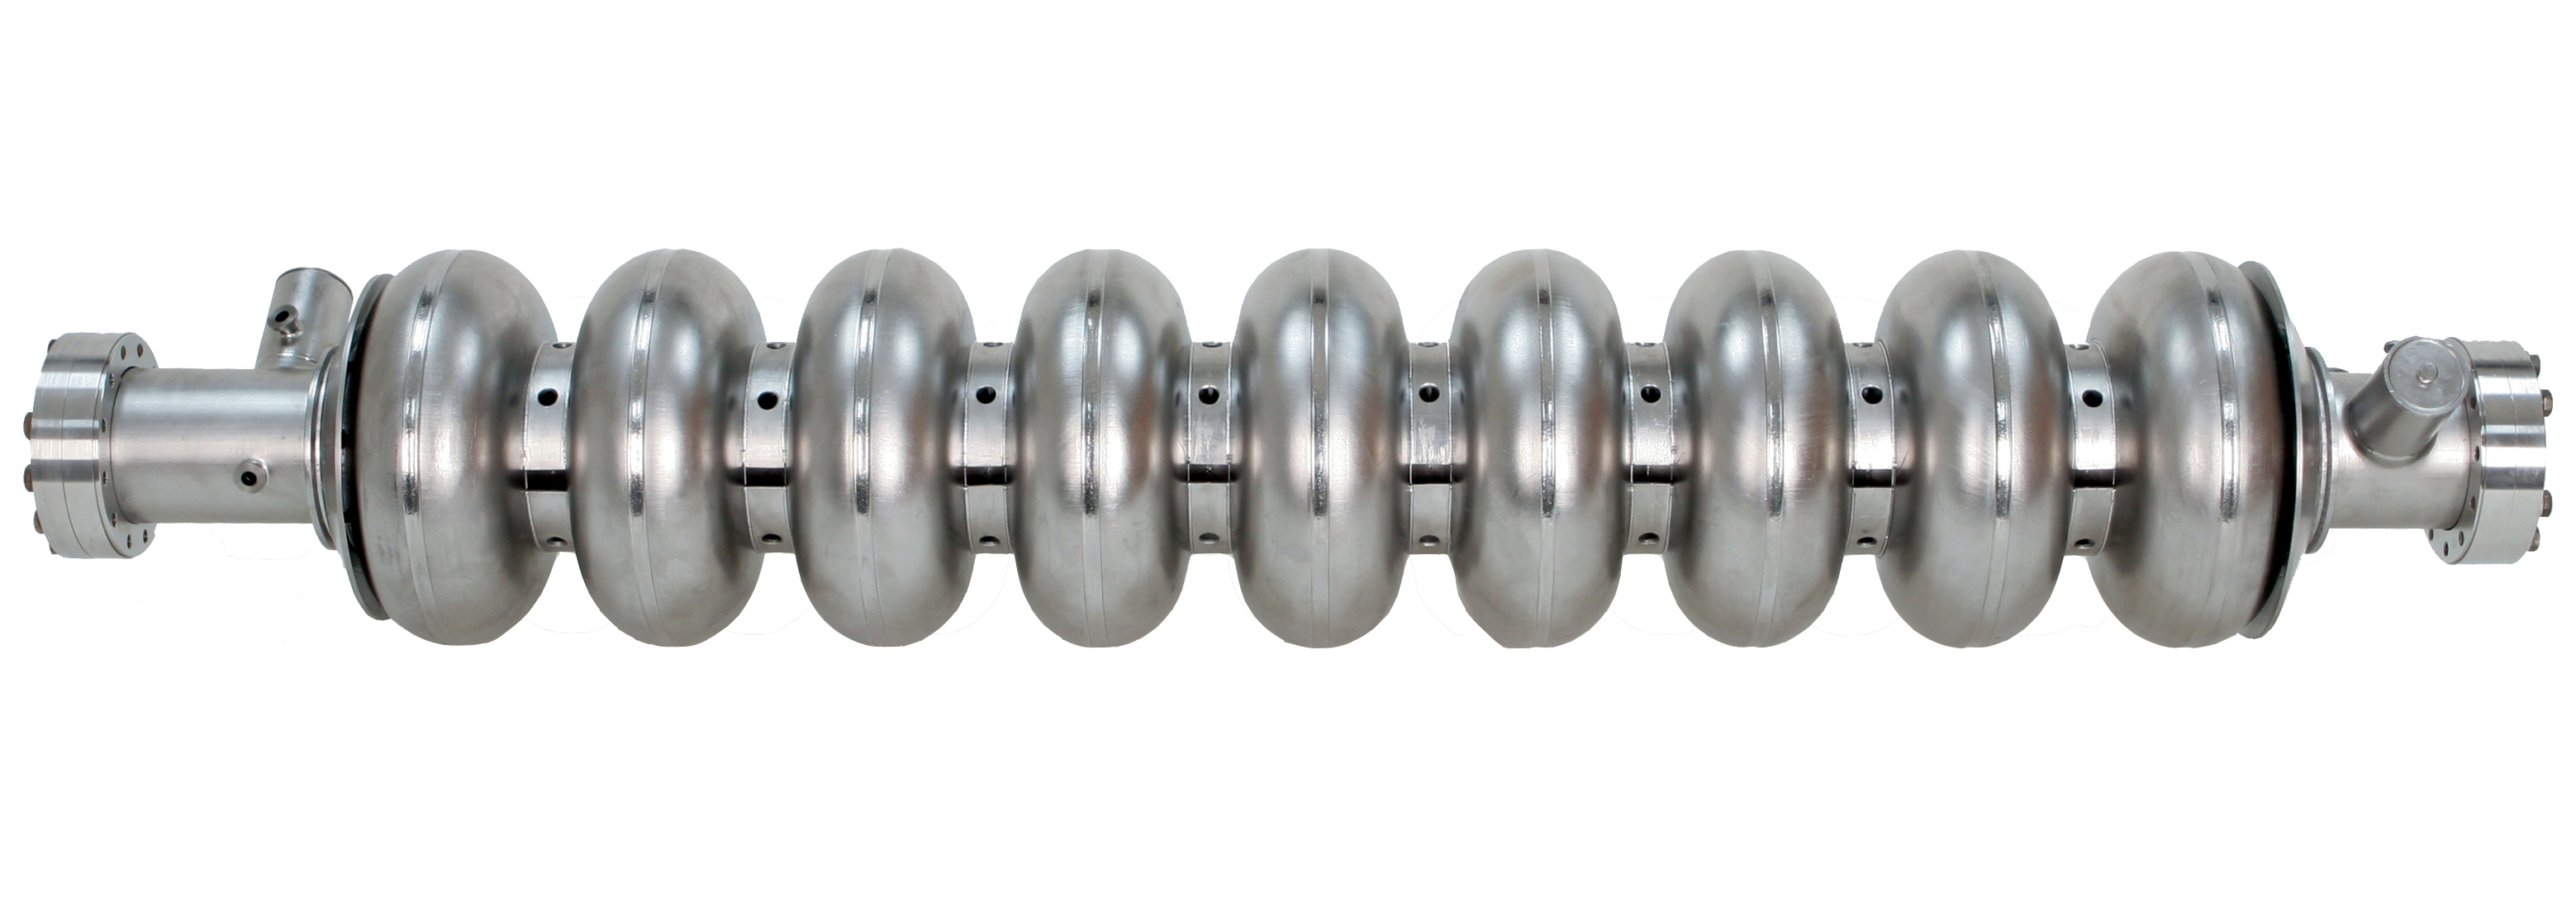
\includegraphics[width=\hsize]{figures/tesla9cell-cavity-2}
\caption{A $1.3\,{\mathrm{GHz}}$ superconducting niobium nine-cell cavity.
}
% Figure from TDR Executive Summary
% https://svnsrv.desy.de/k5websvn/wsvn/General.ilctdr/tags/FormOne-Print-Release/tdres/accel/figs/tesla9cell-cavity-2.jpg
\label{fig:tesla-cavity}
\end{figure}

After welding, the inner surface of the cavity must be prepared.
The process is designed to remove material damage incurred by chemical procedures during the fabrication process, remove chemical residues from earlier production steps, remove hydrogen in the bulk niobium from earlier chemical processing, and remove and particulate contamination.
in a last step, the cavity is closed to form a hermetically sealed structure ready for transport.
The treatment steps involve a series of rinses with ethanol or high pressure water, annealing in a high purity vacuum furnace at \siunit{800^\circ}{C} and \siunit{120^\circ}{C}, and electro polishing or buffered chemical polishing.
The recipe for the surface preparation has been developed over a long time and still subject to optimisation, as it is a major cost driver for the cavity production and largely determines the overall performance and yield of the cavities.
In particular the electro polishing steps are complicated and costly, as they require complex infrastructure and highly toxic chemicals.

{\it 
ADD SOMETHING ABOUT QA AND RETREATMENT HERE.

EXPLAIN INTEGRATION WITH MAGNETIC SHIELD AND TUNER}
 


\subsubsection{Power Coupler}


\subsubsection{Cryomodules}

\begin{figure}[htbp]
   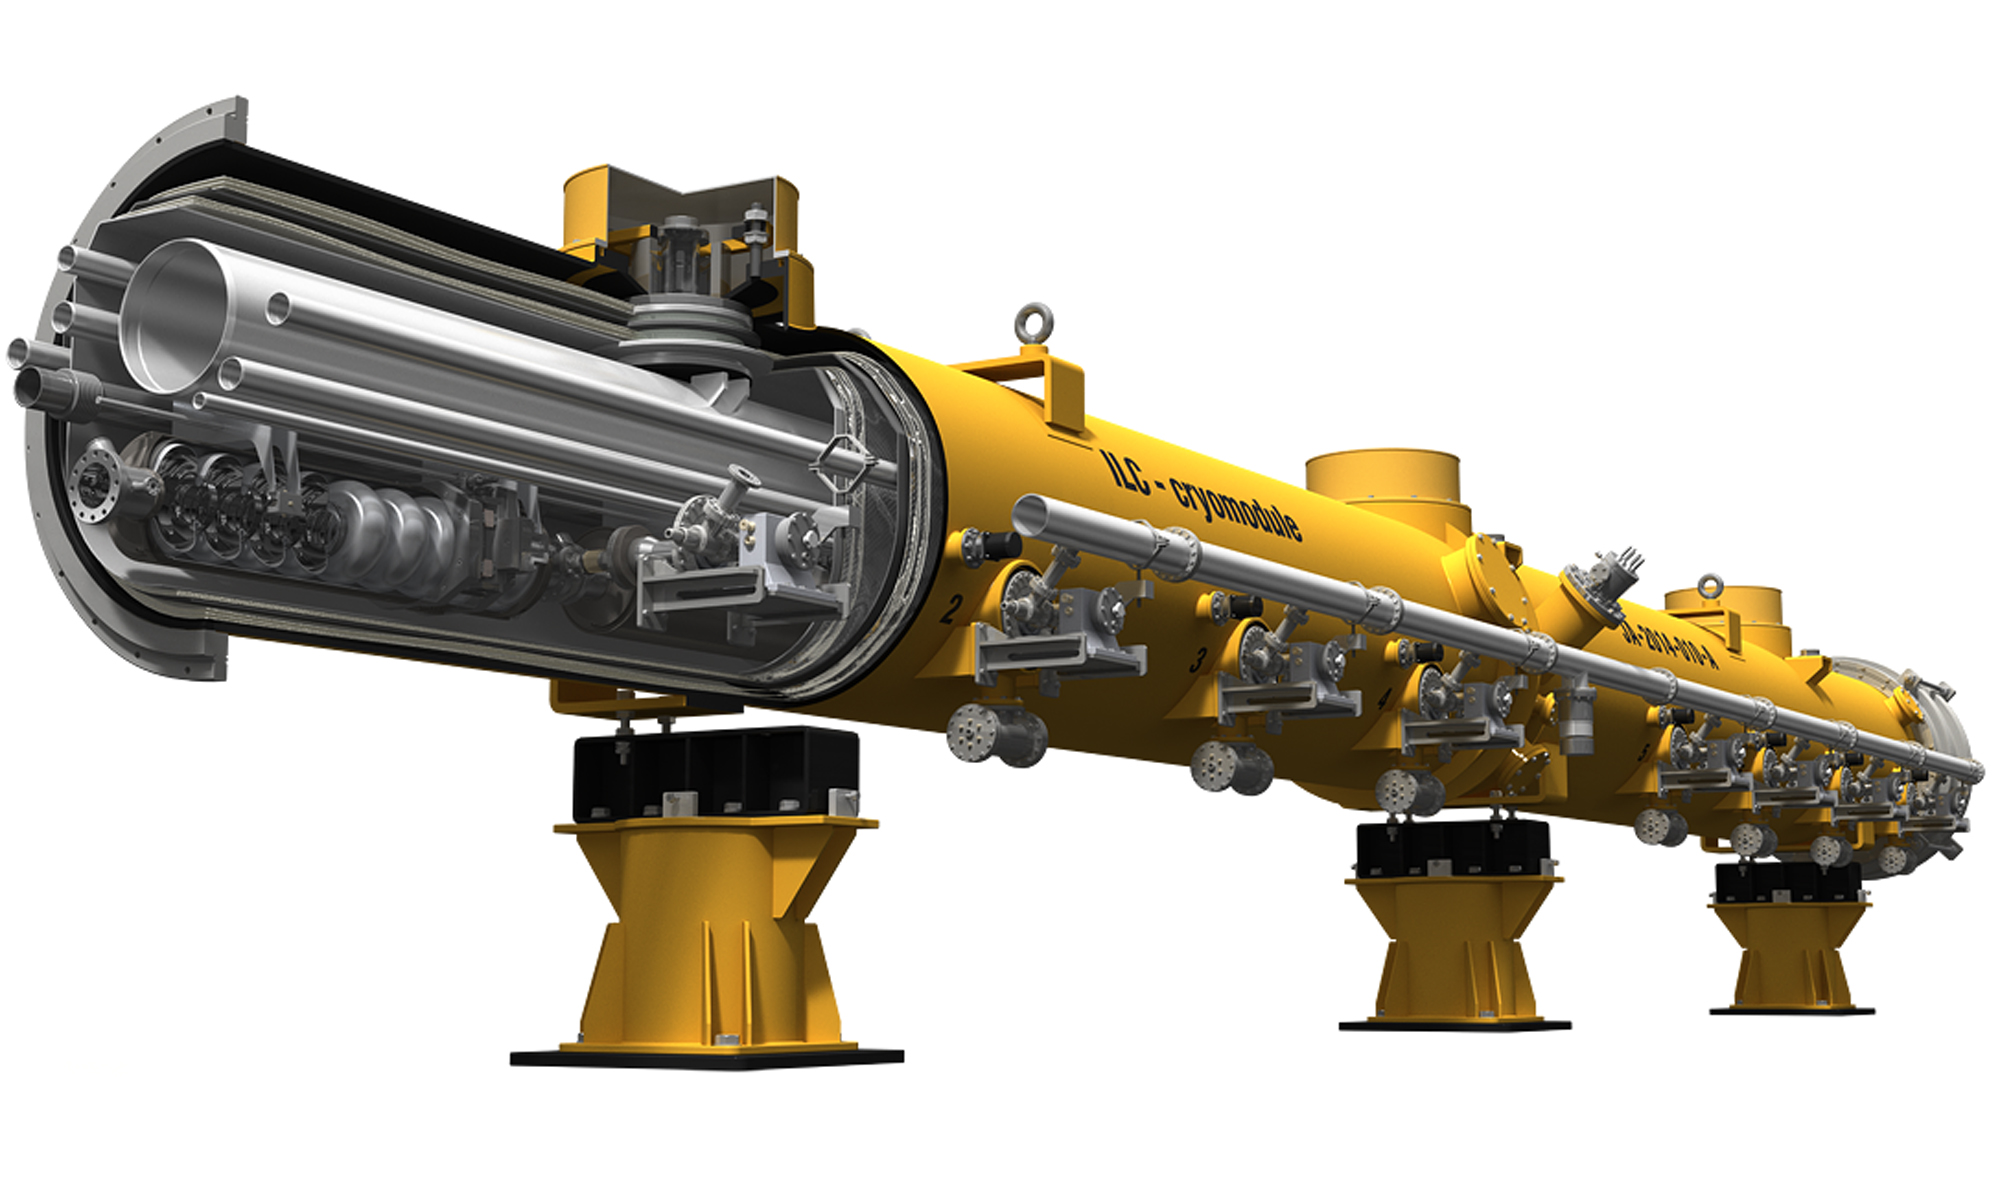
\includegraphics[width=\hsize]{figures/10_ILC_cryomodule}
\caption{An ILC type cryomodule. \copyright Rey.Hori/KEK.}
% Figure from Rey.Hori - check copyright!
% http://www.linearcollider.org/images/pid/1000890/gallery/10_ILC_cryomodule.jpg
\label{fig:crymodule}
\end{figure}



\subsubsection{High-Level Radiofrequency}


\subsubsection{Cryogenics}


\subsubsection{Existing and Future Facilities}

\subsubsection{Series Production and Industrialisation, Worldwide and in Europe}

Due to the construction of the European XFEL, the industrial basis for the key SCRF components is broad and mature, in particular in Europe.
Europe has a leading supplier for raw material. 
In all three regions (Europe, America, Asia), several vendors for cavities have been qualified for ILC type cavities, and provided cost estimates in the past.
Two leading cavity vendors are European companies that have profited from large scale production of cavities for XFEL; 
both have won contracts for LCLS-II as a consequence, which illustrates the potential to create revenue from outside Europe should the ILC be built.
RF couplers have also been successfully produced by European and  American vendors for the XFEL and LCLS-II projects.

ILC/TESLA type cryo modules have been built in laboratories around the world (DESY, CEA in Europe, FNAL and JLAB in America, KEK in Asia).
Series production has been established in America at Fermilab and JLAB for LCLS-II,.
The largest series production was conducted by CEA in France, again for the XFEL, with the assembly of \num{103} cryo modules in total by an industrial partner under the supervision of CEA personnel, with a final throughput of one cryo module produced every four working days.

ILC type, pulsed \siunit{10}{MW} klystrons are commercially available from two vendors in Japan and Europe.

For XFEL, China has been a supplier for niobium raw material and cryomodule cold masses (the cryostat with internal insulation and tubing).
For the planned SCLF project in Shanghai, China has started to develop cavity and cryo module production capabilities, which will further broaden the worldwide production capabilities for SCRF components.
This reduces the risk that prices are pushed up by a monopoly of manufacturers for a large scale order of components as required for the iLC.

Overall, European industry is well prepared to produce the high-tech, high-value SCRF components needed for the ILC, which would likely constitute largest fraction of any European in-kind contribution (IKC) to the ILC, at very competitive prices.
Thus, expenditure for the European IKC will likely stay in Europe, with an excellent chance to stay within the price range assumed in the value estimate.
Moreover, European companies are well poised to win additional contracts from other regions, increasing the economic benefit for Europe from an ILC project.

\subsubsection{Cost Reduction R\&D}

The niobium raw material and preparation of sheets  are a significant cost driver; R\&D is underway to re-evaluate the stringent limits on impurities, especially of tantalum, and the demand for a high residual resistivity ratio $RRR > 300$, to reduce the raw material cost. 
Together with direct slicing of discs from large niobium ingots, without rolling, forging and grinding or polishing steps, the cost for niobium sheets has the potential to be reduced by $50\,\%$~\cite{Evans:2017rvt}.



%===============================================================================

\subsection{Accelerator Design}

{\it 
Description of accelerator design - 5 pages 

Table: Accelerator parameters (250 GeV initial stage, energy and luminosity upgrades
}



\subsubsection{Electron and Positron Sources}

The electron and positron sources are designed to produce \siunit{5}{GeV} beam pulses with the a bunch charge that is $50\,\%$ higher than the design bunch charge of \siunit{3.2}{nC} ($\siunit{2\cdot 10^{10}}{e}$), in order to have sufficient reserve to compensate  any unforeseen inefficiencies in the beam transport.
in the baseline design, both sources produce polarized beams with the same time structure as the main beam, i.e. $1312$ bunches in a $\siunit{727}{\mu s}$ long pulse.

The electron source design~\cite{Adolphsen:2013kya} is based on the SLC polarized electron source, which has demonstarted that the bunch charge, polarisation and cathode lifetime parameters are feasible.
Only the long bunch trains of the ILC require a newly developed laser system and powerful preaccelerator structures, for which preliminary designs are available.
The design foresees a Ti:sapphire laser impinging on a photocathode based on a strained GaAs/GaAsP superlattice
structure, which will produce electron bunches with an expected polarisation of \SIunit{85}{\%},
sufficient for \SIunit{80}{\%} beam polarization at the interaction point, as demonstrated at SLAC~\cite{Alley:1995ia}.

The positron source poses a larger challenge. 

In the baseline design, hard gamma rays are produced in a helical undulator driven by the main electron beam, which are converted to positrons in a rotating target.
Positrons are captured in a flux concentrator or a quarter wave transformer, accelerated to \siunit{400}{MeV} in two normal conducting preaccelerators followed by a superconducting accelerator very similar to the main linac, before they are injected into the damping rings at \siunit{5}{GeV}.
Compared to planar undulators, the helical undulators produce twice as many photons, and with circular polarisation, which is transferred to the positrons produced in the target.
The positron polarisation thus achieved is $30\,\%$.
The E-166 experiment at SLAC has successfully demonstrates this concept  \cite{Alexander:2009nb}, albeit at intensities much lower than foreseen for the ILC. 
Technological challenges of the undulator source concept are the target heat load, radiation load in the flux concentrator device, and dumping the high intensity photon beam remnant.

As an alternative, an electron driven positron source concept has been developed.
In the electron driven scheme, a \siunit{3}{GeV} electron beam from a dedicated normal conducting linac produces positrons in a rotating target.
The electron drive beam, being independent from the main linac, has a completely different time structure. 
Positrons are produced in $20$ pulses at \siunit{300}{Hz} with $66$ bunches each, i.e., it takes about \siunit{67}{ms} to produce all positrons for a single Main Linac pulse with its $1312$ bunches, compared to \siunit{0.8}{ms} for the undulator source.
This different time structure reduces spreads the heat load on the target over a longer time, allowing a target rotation speed of only \siunit{5}{m/s} rather than \siunit{100}{m/s}, which reduces the engineering complexity of the target design, in particular the vacuum seals of the rotating parts.
Although not free from its own engineering challenges, such as the high beam loading in the normal conducting cavities, the electron driven design is currently considered to be a low risk design that is sure to work.

Aside from the low technical risk, the main advantage of the electron driven design is the independence of positron production and electron main linac operation, which is an advantage for accelerator commissioning and operation in general.
In particular, electron beam energies below \siunit{120}{GeV} for operation at the $Z$ resonance or the $WW$ threshold would be no problem.
The undulator source, on the other hand, offers the possibility to provide beams at the maximum repetition rate of \siunit{10}{Hz} given by the damping time in the damping rings of \siunit{100}{ms}, whereas the electron driven scheme is limited to \siunit{6}{Hz} due to the additional \siunit{66}{ms} for positron production.
The main difference, however, between the concepts is the positron polarisation offered by the undulator source, which adds significantly to the physics capabilities of the machine, as discussed elsewhere in this report. 

Both concepts have been reviewed recently \cite{PWG:2018a} inside the ILC community, with the result that both source concepts appear viable, with no known show stoppers, but require some more engineering work. 
The decision on the choice will be taken once the project has been approved, based on the physics requirements, operational aspects, and technological maturity and risks. 


\begin{table*}
\begin{tabular}{lccccc}
Quantity & Symbol & Unit & Initial &  \multicolumn{2}{c}{Upgrades} \\
\hline
Centre of mass energy & $\sqrt{s}$ & ${\mathrm{GeV}}$ & $250$ & $500$ & $1000$ \\
Luminosity & \multicolumn{2}{c}{${\mathcal{L}}$ $10^{34}{\mathrm{cm^{-2}s^{-1}}}$} & $1.35$ & $1.8$ & $4.9$ \\
Repetition frequency &$f\sub{{rep}}$ & ${\mathrm{Hz}}$  & $5$ & $5$ & $4$ \\
Bunches per pulse  &$n\sub{{bunch}}$ & 1  & $1312$ & $1312$ & $2450$ \\
Bunch population  &$N\sub{{e}}$ & $10^{10}$ &$2$ & $2$ & $1.74$ \\
Linac bunch interval & $\Delta t\sub{{b}}$ & ${\mathrm{ns}}$ & $554$ & $554$ & $366$ \\
Beam current in pulse & $I\sub{{pulse}}$ & ${\mathrm{mA}}$& $5.8$ & $5.8$ & $7.6$  \\
Beam pulse duration  & $t\sub{{pulse}}$ & ${\mathrm{\mu s}}$ &$727$ & $727$ & $897$ \\
Average beam power  & $P\sub{{ave}}$   & ${\mathrm{MW}}$ & $5.3$   &$10.5$  & $27.2$ \\  
Norm. hor. emitt. at IP & $\gamma\epsilon\sub{{x}}$ & ${\mathrm{\mu m}}$& $5$ & $10$ & $10$  \\ 
Norm. vert. emitt. at IP & $\gamma\epsilon\sub{{y}}$ & ${\mathrm{nm}}$ & $35$ & $35$ & $35$ \\ 
RMS hor. beam size at IP  & $\sigma^*\sub{{x}}$ & ${\mathrm{nm}}$  & $516$ & $474$ & $335$ \\
RMS vert. beam size at IP &$\sigma^*\sub{{y}}$ & ${\mathrm{nm}}$ & $7.7$  & $5.9$ & $2.7$ \\
Site AC power  & $P\sub{{site}}$ &  ${\mathrm{MW}}$ & $129$ & $163$ & $300$ \\
Site length & $L\sub{{site}}$ &  ${\mathrm{km}}$ & $20.5$ & $31$ & $40$ \\
\end{tabular}
\caption{Summary table of the ILC accelerator parameters in the initial $250\,{\mathrm{GeV}}$ staged configuration
and possible upgrades.
\label{tab:ilc-params}}
\end{table*}


\subsubsection{Damping Rings}

{\it Mention ATF

Nomura issues: Feedback system

}

The ILC comprises two oval damping rings of \siunit{3.2}{km} circumference, sharing a common tunnel in the central accelerator complex.
The damping rings reduce the horizontal and vertical emittance of the beams by up to five orders of magnitude\footnote{The vertical emittance of the positrons is reduced from $\epsilon_{\mathrm{y}} \approx 0.8\,{\mathrm{\mu m}}$ to $10\,{\mathrm{pm}}$.} within a time span of only \siunit{100}{ms}, to provide the low emittance beams required at the interaction point. 
Both damping rings operate at an energy of \siunit{5}{GeV}.
To achieve the high synchrotron radiation damping required by the low damping time,  the rings are equipped with $54$ superconducting wigglers in each ring, bringing the energy loss per turn up to $7.7\,{\mathrm{MV}}$.
This requires in $3.3\,{\mathrm{MW}}$ RF power per beam at the design current of $390\,{\mathrm{mA}}$, which actually surpasses the RF power of $2.6\,{\mathrm{MW}}$ needed to accelerate the beams in the main linacs at \siunit{125}{GeV} beam energy.

Compared to today's fourth generation light sources, the target value for the beam emittance ($\siunit{4}{\mu m}$/\siunit{20}{nm} for the normalised horizontal / vertical beam emittance) is low, but not a record value, and thus considered to be a realistic goal.

 

\subsubsection{Low Emittance Beam Transport}

\subsubsection{Bunch Compressors and Main Linac}

{\it Figure: ML cross section}

\subsubsection{Beam Delivery System and Machine Detector Interface}

{\it Stress ATF2, FONT (maybe SLAC FFTB)

Nomura issues: Dumps, crab cavities

Mention beam dumps as well}

%===============================================================================

\subsection{Upgrade Options}

{\it 
Description of luminosity and energy upgrades - 1 page }


%===============================================================================

\subsection{Civil Engineering and Site}

{\it 
Description of Civil engineering plans and Kitakami site - 3 pages

Figures: Kitakami Site, Kitakami site cross section}

\begin{figure}[htbp]
   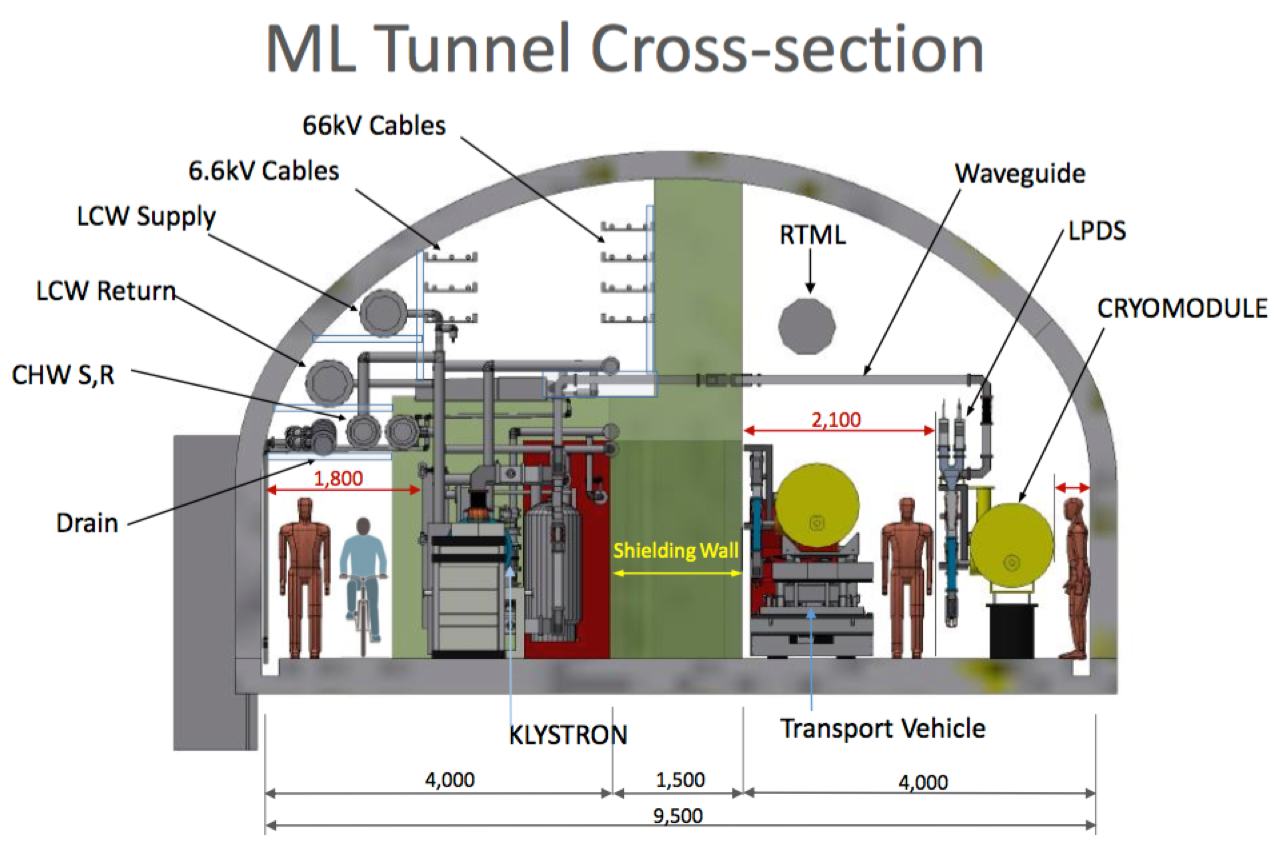
\includegraphics[width=\hsize]{figures/ML-cross-section}
\caption{Cross section through the Main Linac tunnel.}
\label{fig:ml-tunnel}
\end{figure}


\begin{figure}[htbp]
   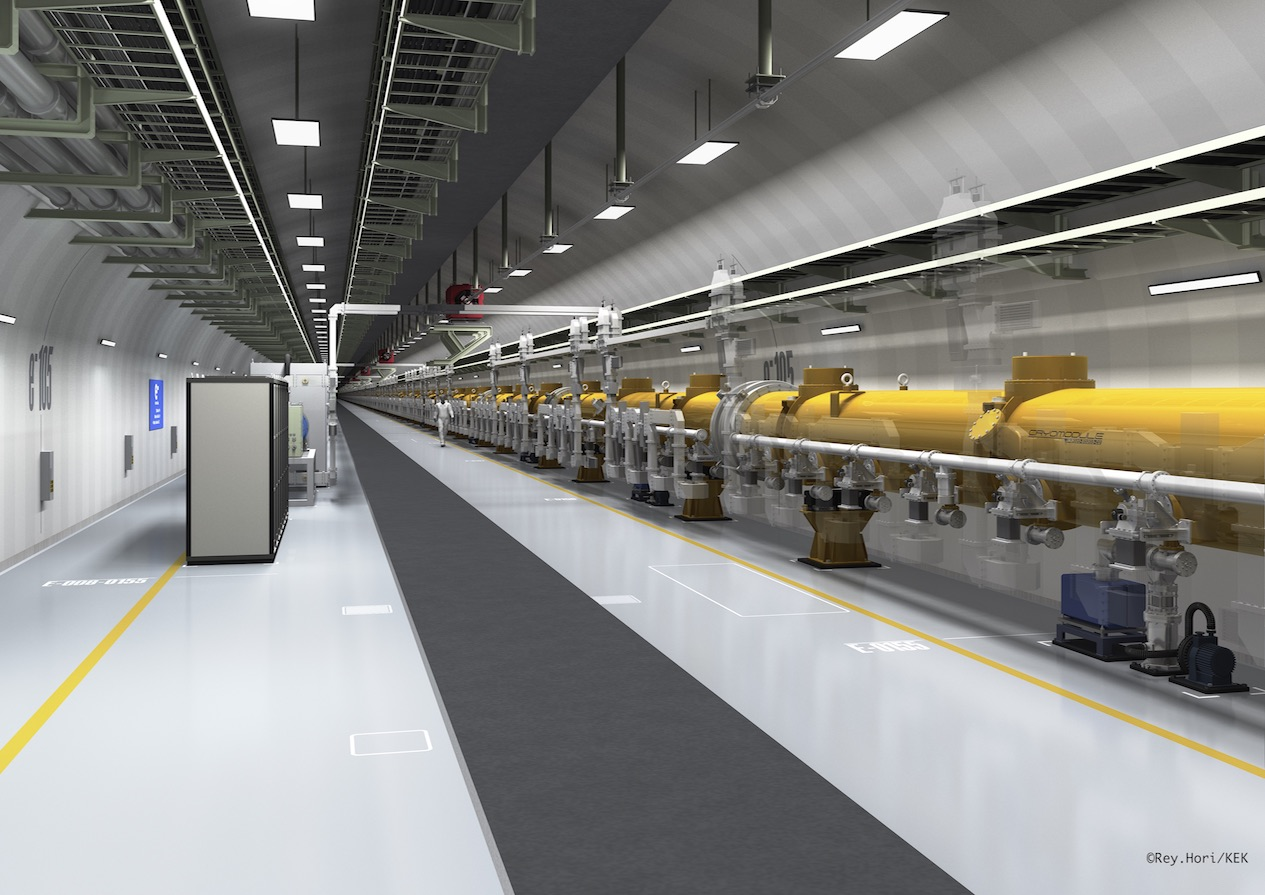
\includegraphics[width=\hsize]{figures/ILC2016_tunnel_A1_160826-low4}
\caption{Artist's rendition of the ILC Main Linac tunnel. The shield wall in the middle has been removed.
\copyright Rey.Hori/KEK.}
\label{fig:ilc-tunnel}
\end{figure}

\begin{figure}[htbp]
   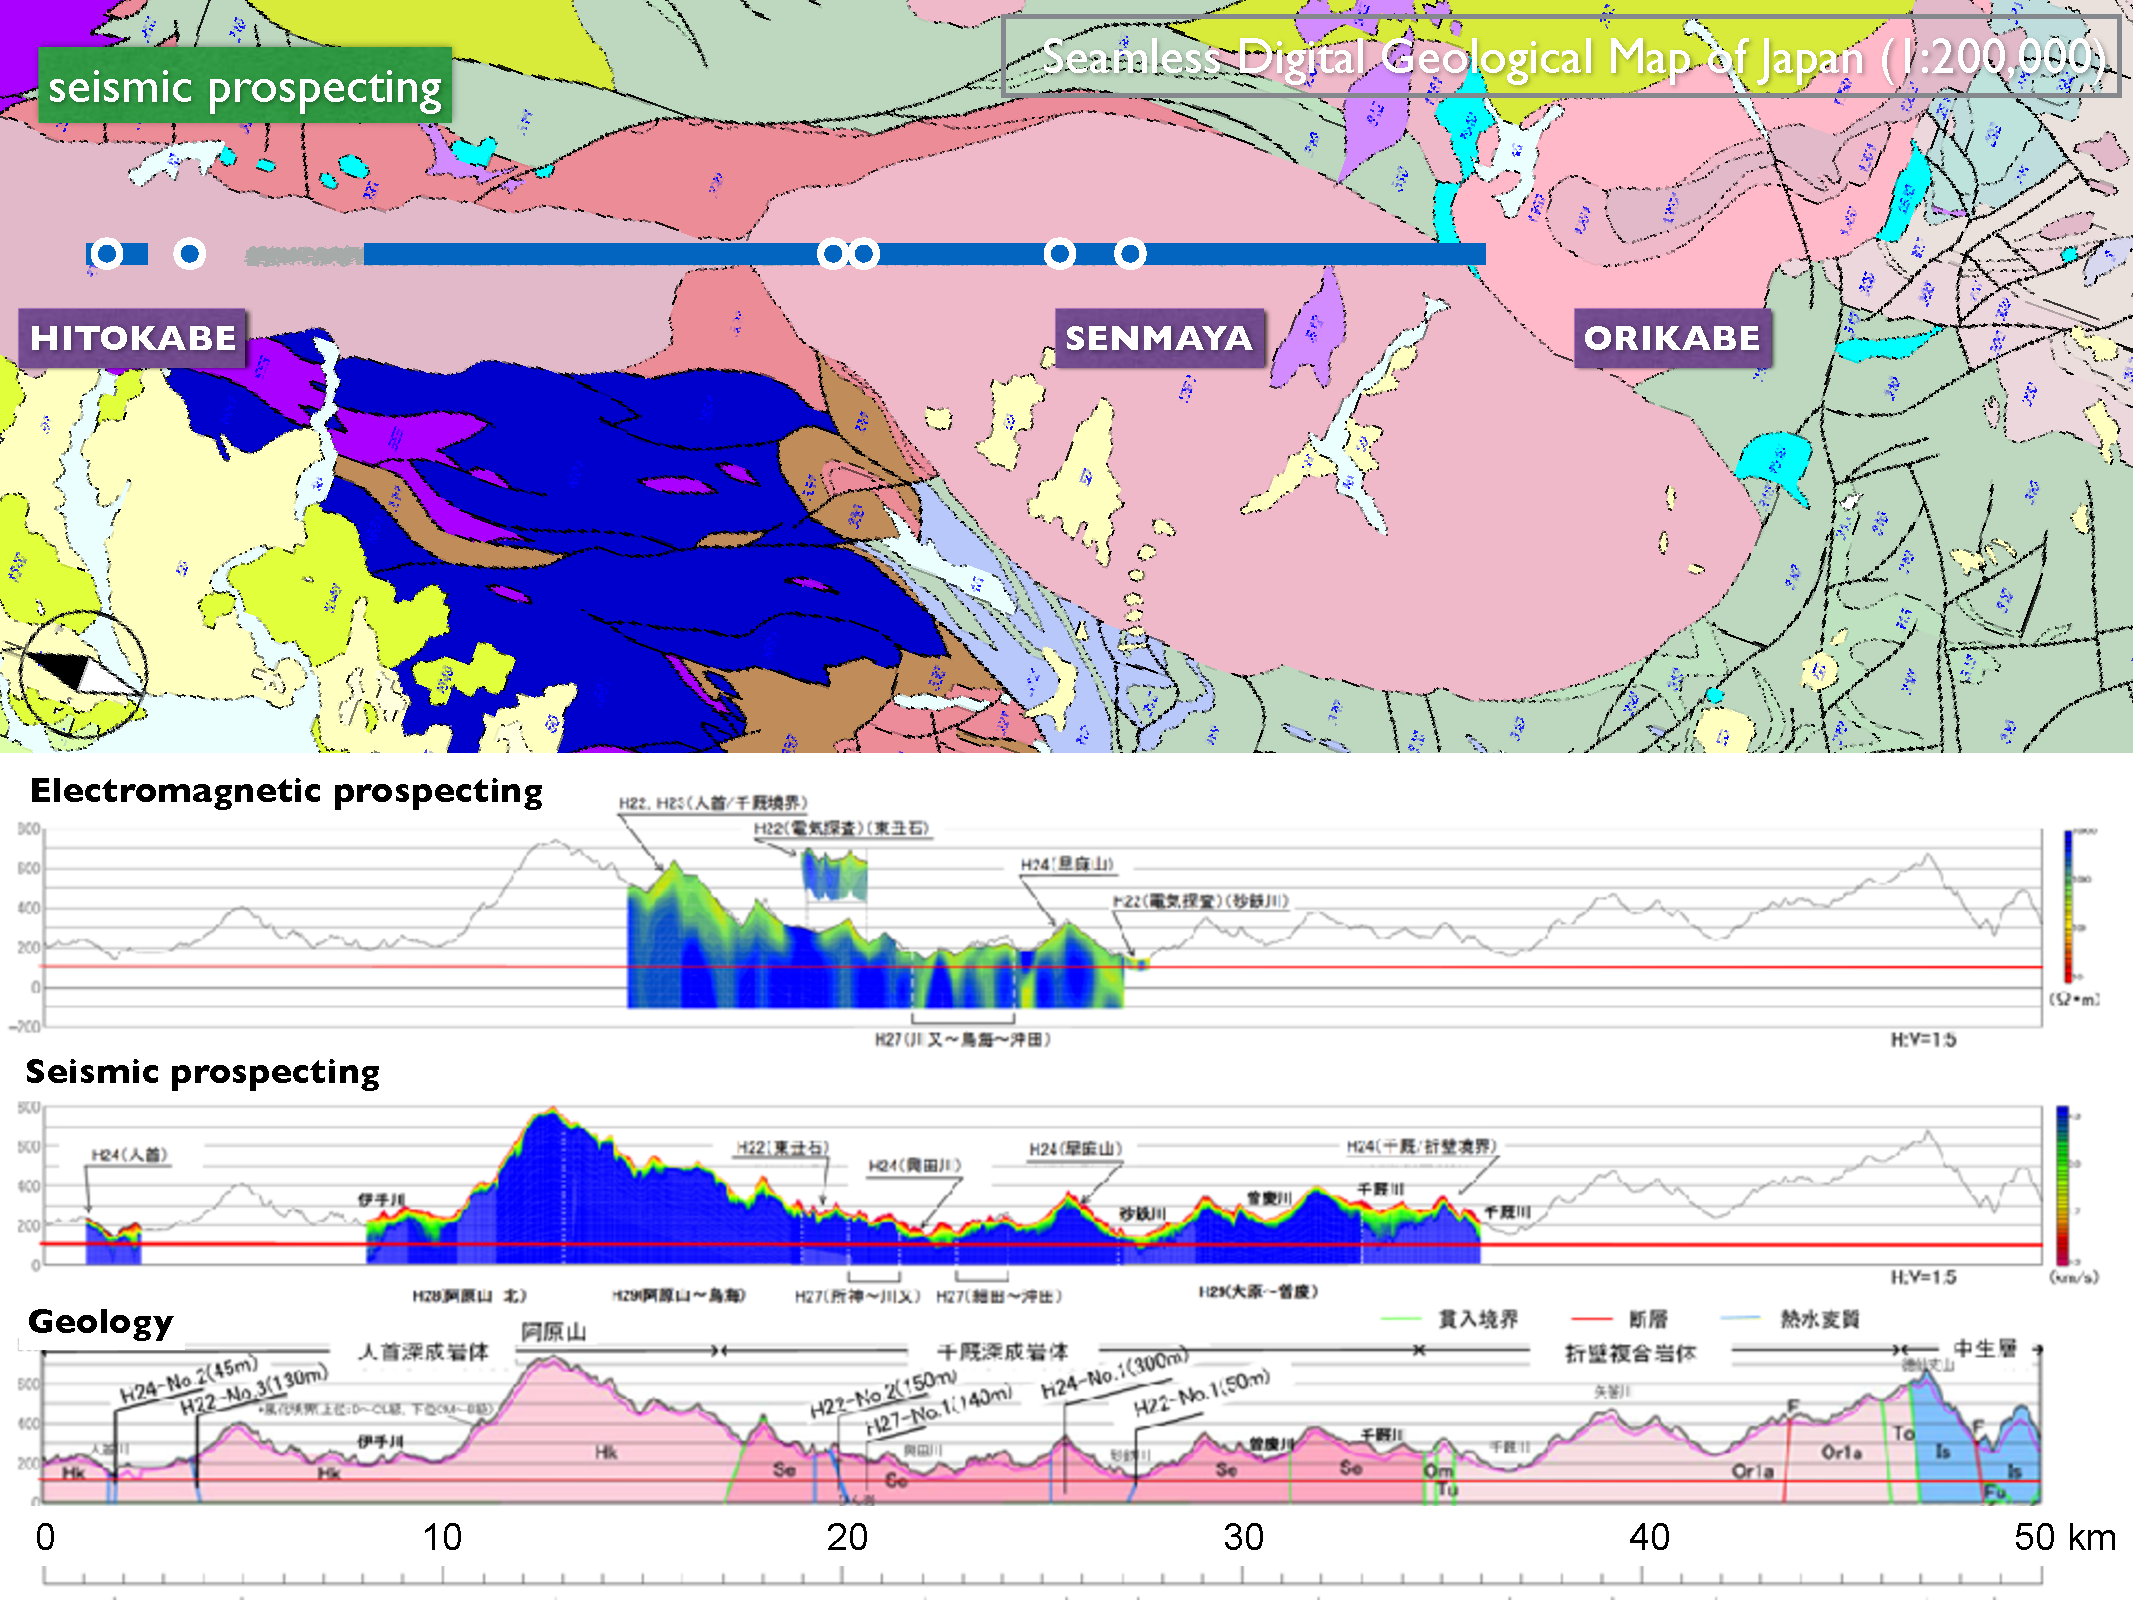
\includegraphics[width=\hsize]{figures/Kitakami_Geology}
\caption{Geological situation at the Kitakami site.}
\label{fig:kitakami-geology}
\end{figure}


%===============================================================================

\subsection{Cost and Schedule}

{\it 
Description of Cost estimate and schedule - 1 page 

include human resources, cost reduction effect by R\&D, operating costs
}



